\section{Descrizione del sistema}
\label{sec:sistema-reale}
Il sistema è mostrato in \autoref{fig:foto-sistema}.
Per costruirlo ho usato componenti meccaniche ed elettroniche
disponibili commercialmente.
Tutti i supporti di colore blu sono stati
realizzati con la stampa-3D. Segue una lista dettagliata di tutte le componenti.

\begin{figure}[H]
    \centering
    \fbox{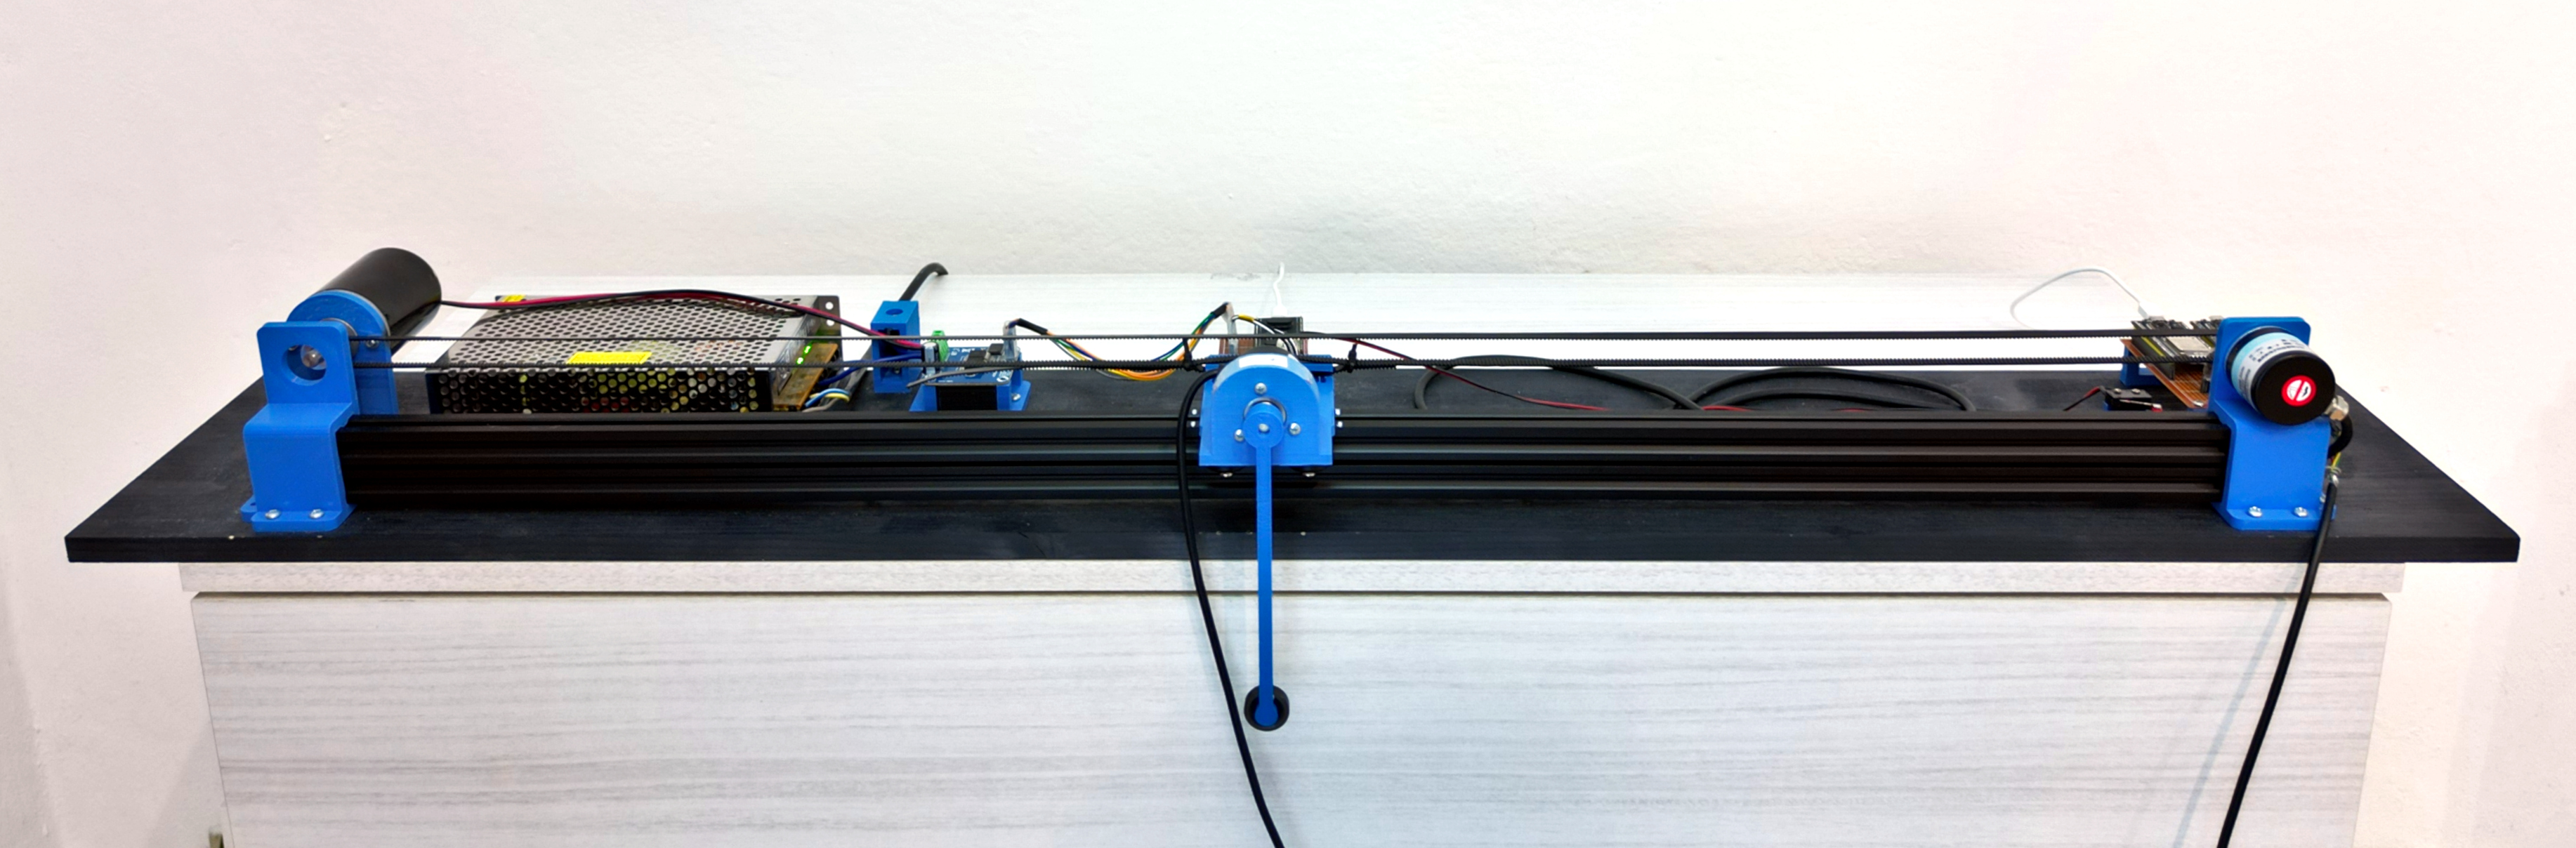
\includegraphics[width=.98\textwidth]{assets/pendolo-down}}
    \caption[Foto del sistema]{Foto del sistema che ho costruito, spento.}
    \label{fig:foto-sistema}
\end{figure}

\subsection{Componenti meccaniche}
\label{subsec:componenti-meccaniche}
Ho usato prevalentemente componenti standard di \emph{OpenBuilds}~\cite{openbuilds},
assieme a supporti realizzati con la stampa-3D.
Tutte le componenti sono montate su una base di legno.

Il design meccanico è dettato dalla necessità di avere un vincolo
lineare per il carrello
che riduca il più possibile tutti gli effetti non modellabili.
Il vincolo è dato da una rotaia, realizzata con un profilato in alluminio
\emph{V-Slot} lungo $1m$.
Il carrello scorre sulla rotaia, supportato da
ruote \emph{Mini-V}.
La forma delle ruote combacia con la forma del profilato,
garantendo un movimento lineare, senza vibrazioni e con basso attrito.
Il dettaglio del carrello è riportato in \autoref{fig:dettaglio-carrello}.

\begin{figure}
    \centering
    \fbox{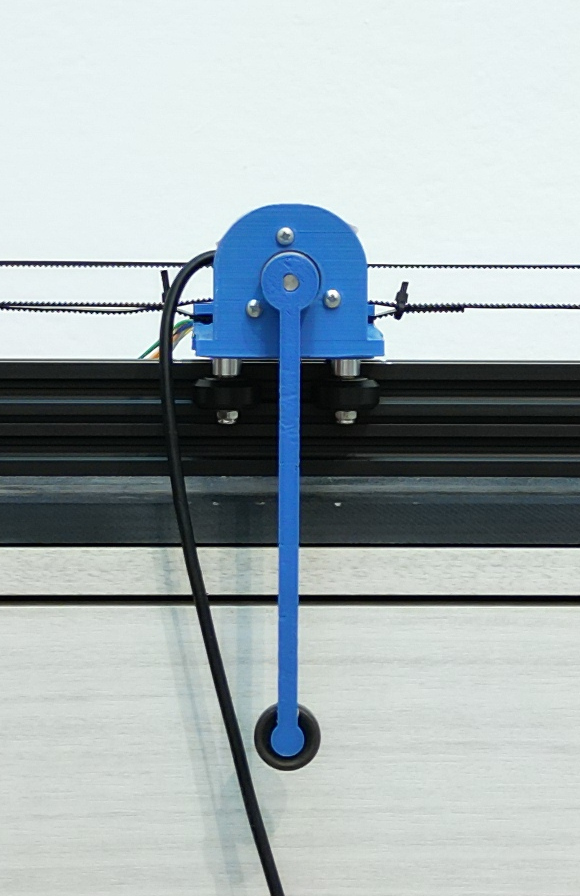
\includegraphics[width=.5\textwidth]{assets/dettaglio-carrello}}
    \caption[Dettaglio del carrello]{Dettaglio del carrello. Il pendolo è montato
    su un encoder, fissato al carrello tramite un supporto realizzato con la
    stampa-3D. Il carrello scorre sulla rotaia grazie alle ruote orizzontali.}
    \label{fig:dettaglio-carrello}
\end{figure}

Il carrello è collegato al motore tramite una cinghia dentata \emph{GT-2}.
La cinghia è di gomma con un cuore di metallo, in modo da resistere
alle deformazioni.
La cinghia è mantenuta in tensione dal motore e da un
encoder rotativo, come mostrato in \autoref{fig:dettaglio-motore} e
\autoref{fig:dettaglio-encoder}.
Il motore è un modello \emph{XD-3420}
a spazzole, a corrente continua e con tensione nominale di $12V$.

Sul carrello è montato un secondo encoder rotativo,
che funge da perno per il pendolo.
Il cavo collegato al secondo encoder è lasciato pendere
e ho trascurato il suo effetto sul sistema.

\begin{figure}[h]
    \centering
    \fbox{\includegraphics[width=.8\textwidth]{assets/particolare-motore}}
    \caption[Dettaglio del motore]{Dettaglio di motore e alimentatore.
    Il motore è collegato al circuito \emph{H-Bridge} che, a sua volta, è collegato
    all'alimentatore. Un interruttore permette di disattivare il motore.
    Il motore è collegato direttamente alla cinghia.}
    \label{fig:dettaglio-motore}
\end{figure}
\begin{figure}[h]
    \centering
    \fbox{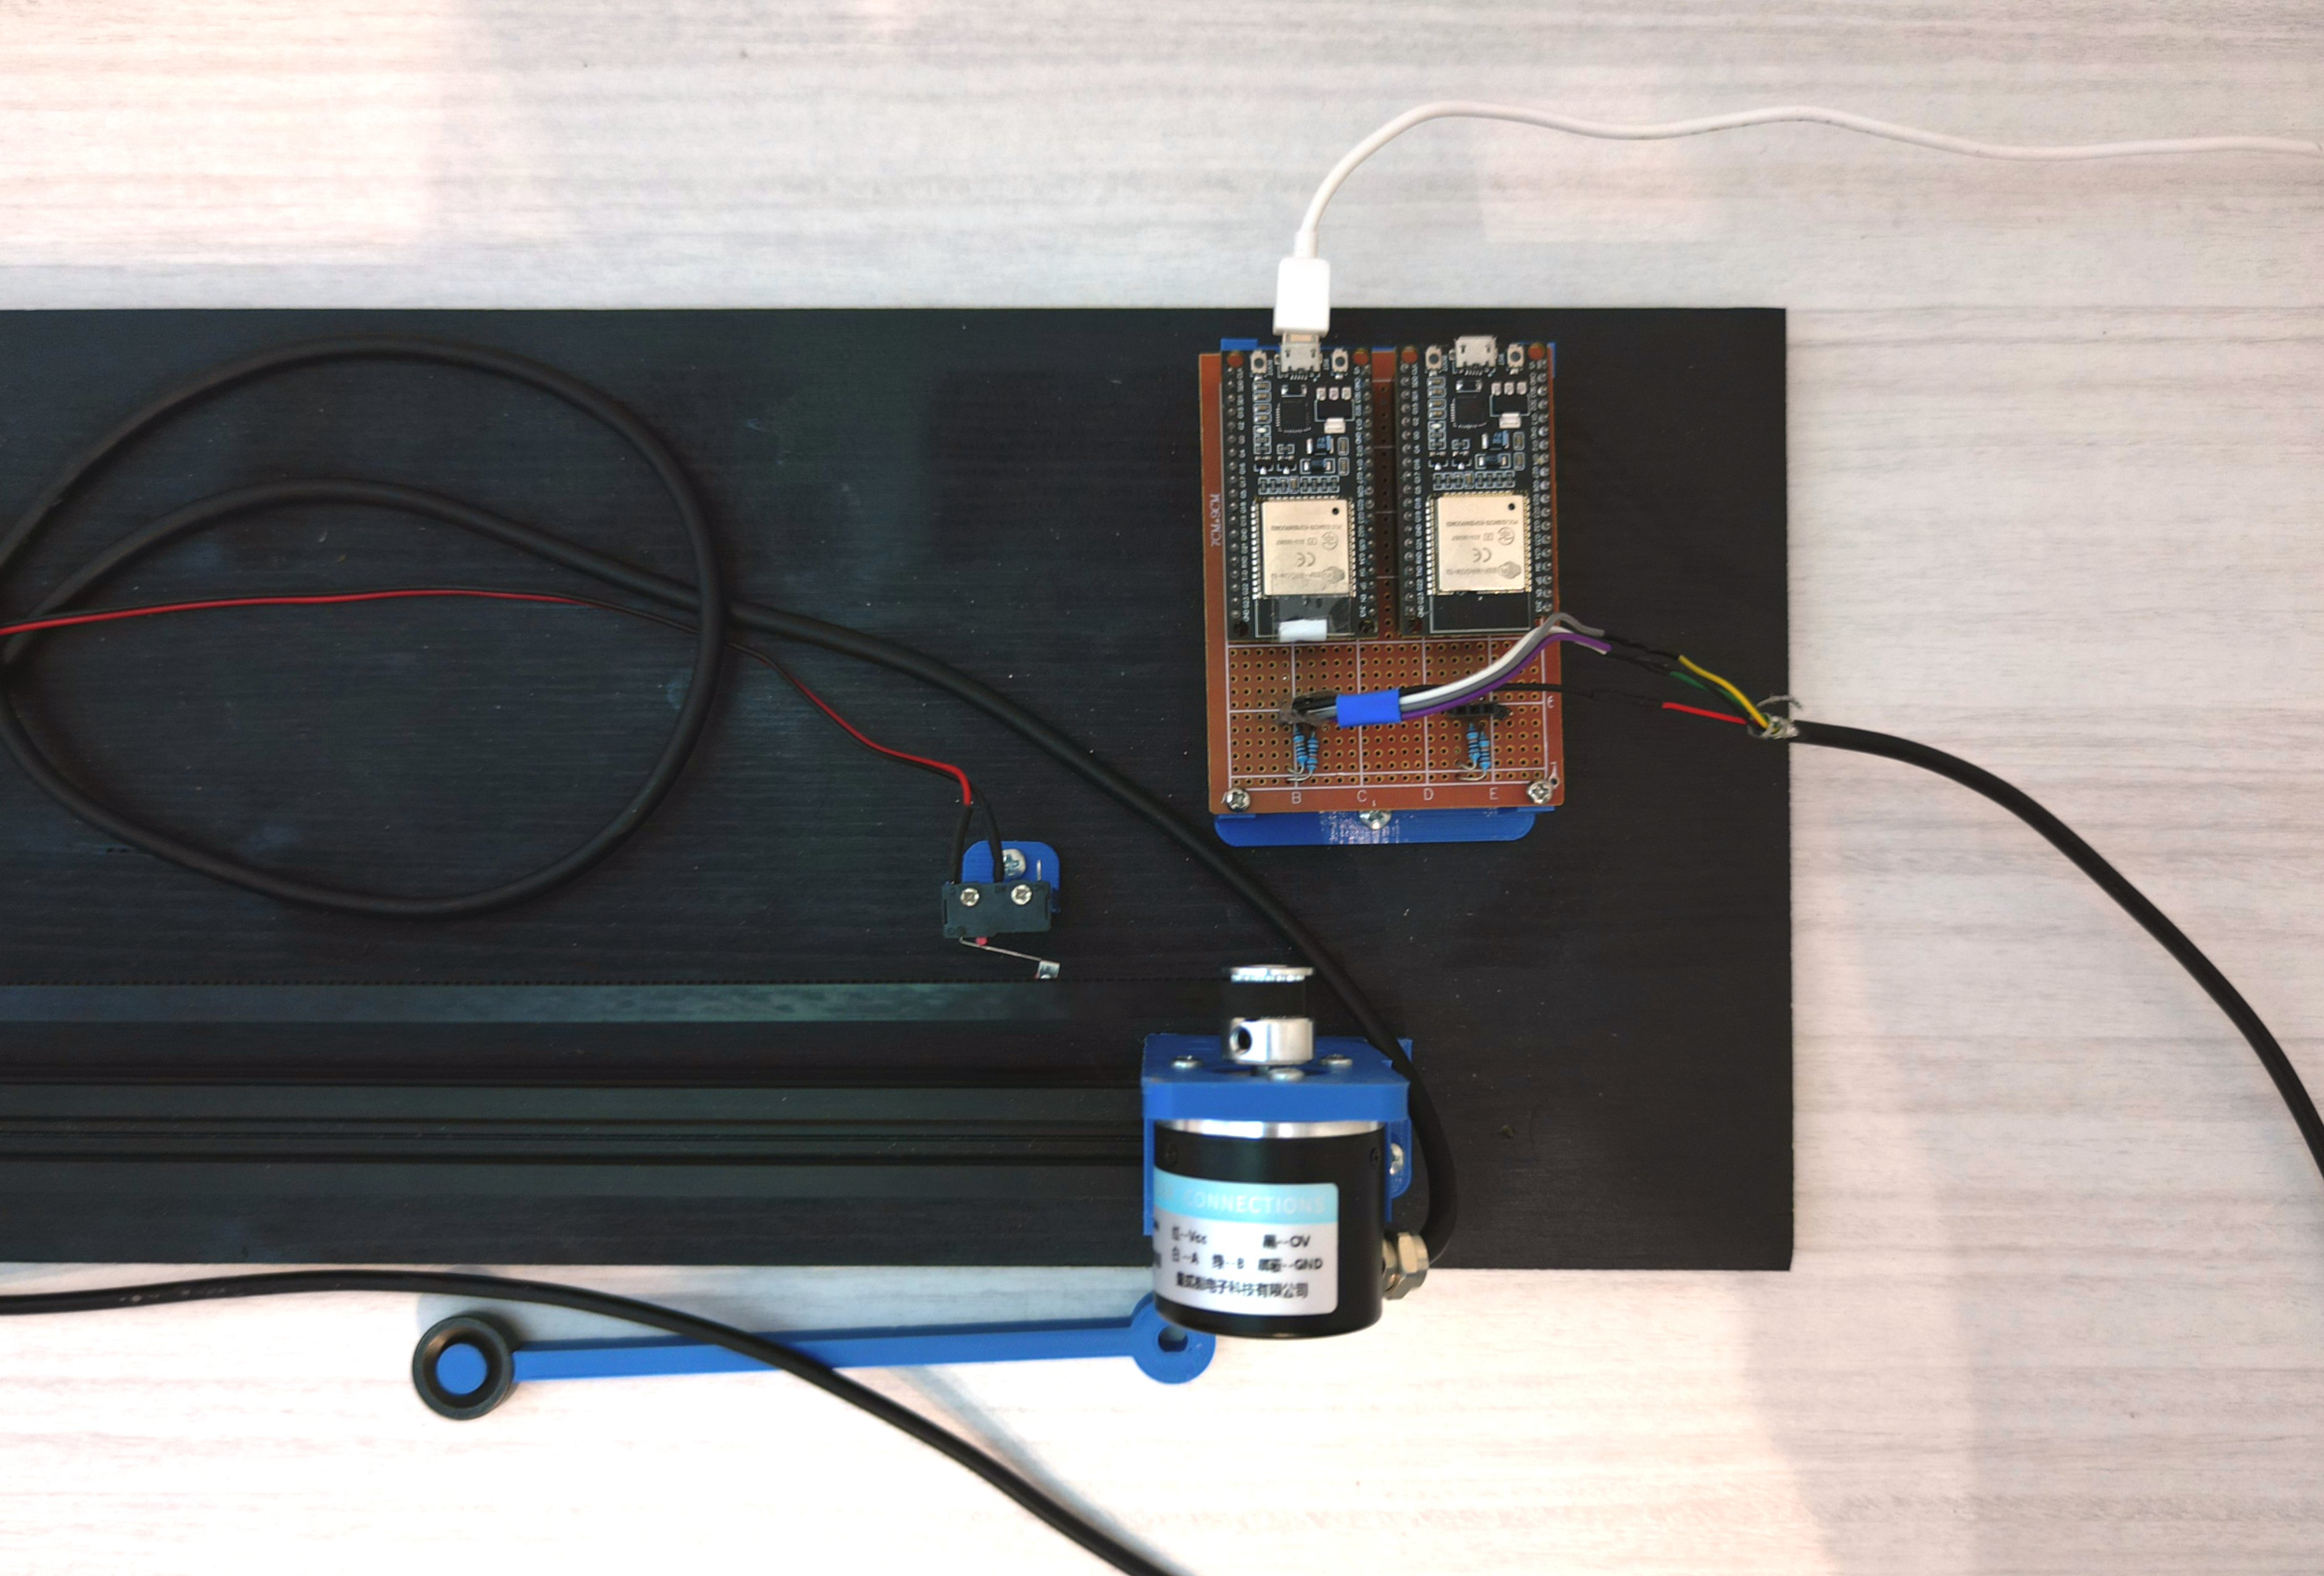
\includegraphics[width=.8\textwidth]{assets/angle-sensor}}
    \caption[Dettaglio encoder]{Dettaglio dell'encoder che misura la posizione.
    La cinghia è tenuta in tensione dall'encoder.
    In alto sono visibili due microcontrollori
    \emph{ESP32}; solo uno di questi è utilizzato.
    }
    \label{fig:dettaglio-encoder}
\end{figure}

\subsection{Componenti elettroniche}
\label{subsec:componenti-elettroniche}

I sensori a cui il sistema ha accesso sono due encoder ottici rotativi\footnotemark,
modello \emph{LPD3806}.
Il primo (\autoref{fig:dettaglio-carrello}) misura langolo del pendolo,
il secondo (\autoref{fig:dettaglio-encoder} la posizione del carrello.
Gli encoder sono incrementali, quindi devono essere azzerati manualmente
ogni volta che si avvia l'esperimento.

\footnotetext{
    Un encoder ottico rotativo è formato da un disco opaco su cui sono
    presenti delle fessure radiali. Una fotocellula è posta ai lati del disco
    e invia un impulso elettrico ogni volta che rileva una fessura. Una
    seconda fotocellula opera allo stesso modo, ma è posizionata in modo che il
    suo segnale sia sfasato rispetto alla prima. Confrontando i segnali delle due
    fotocellule, è possibile ricavare la direzione di rotazione.
}

I dati dei sensori sono letti da due microcontrollori \emph{ESP32}~\cite{esp32}.
I due microcontrollori comunicano usando la tecnologia \emph{ESP-NOW}~\cite{espnow}.
Gli \emph{ESP32} sono dotati di un microprocessore dual-core. Questo mi
permette di riservare un core in ciascun microcontrollore solamente per contare
gli impulsi ricevuti dal rispettivo encoder. Il secondo core è usato, in un caso,
per comunicare i dati all'altro microcontrollore e, nell'altro, per ricevere i dati
e inviare il segnale di controllo al motore. I due microcontrollori sono mostrati
in \autoref{fig:dettaglio-controller} e in \autoref{fig:dettaglio-encoder}.

\begin{figure}[h]
    \centering
    \fbox{\includegraphics[width=.8\textwidth]{assets/particolare-controller}}
    \caption[Dettaglio controller]{Dettaglio
    del microcontrollore che controlla il motore.
    Si vede il collegamento con il circuito
    \emph{H-Bridge}.}
    \label{fig:dettaglio-controller}
\end{figure}

Il motore è alimentato da un alimentatore da $12V$ (\autoref{fig:dettaglio-motore}).
La corrente passa in un circuito a \emph{H-Bridge}, modello \emph{BTS7960},
che permette di cambiare potenza e direzione di rotazione del motore.
La potenza del motore è regolata da un microcontrollore, collegato all'\emph{H-Bridge}, tramite \emph{PWM}\footnotemark. I due microcontrollori sono alimentati da due alimentatori esterni da $5V$. Internamente il sengale \emph{PWM} è rappresentato da un
numero a $8$-bit; il range di valori ammessi per $u$ è quindi $[0, 255] \subset N$.


\footnotetext{
    \emph{PWM} sta per \emph{Pulse Width Modulation}. La tecnica consiste
    nell'inviare al motore una corrente sotto forma di onda quadra.
    L'onda può avere valori di $0V$ o $12V$ e, variando la percentuale di tempo
    che l'onda passa a $12V$, si può variare la potenza del motore.
    Nel mio caso la frequenza dell'onda si è rilevata poco influente sul
    risultato; io ho fissato la frequenza a $500Hz$.
}

Nel sistema non è presente un sensore di corrente in ingresso al motore.
Questo è il motivo per cui nel paragrafo~\ref{subsec:modello-motore} ho limitato
il mio studio al regime stazionario.

\subsection{Dati in uscita dai sensori}
Il microcontrollore che si occupa di controllare il motore riceve i dati
aggiornati dei sensori ogni $2ms$.
Per evitare di sovraccaricare il processore, il segnale di controllo
del motore viene aggiornato una volta ogni $5ms$ e i dati del sistema vengono
trasmessi a un eventuale computer collegato solo una volta ogni $25ms$.
Nonostante il segnale di controllo non sia continuo, l'intervallo temporale
tra un segnale e il successivo è abbastanza piccolo da poterlo approssimare come
tale.
Se così non fosse, sarebbe necessario discretizzare
il modello secondo la ~\eqref{eq:bdequalsint} .

Preciso inoltre che, mentre i dati per $q$ e $\theta$ sono presi esattamente
come escono dai sensori, per i dati di $\dot q$ e $\dot \theta$ viene presa
la media mobile degli ultimi tre punti, in modo da ridurre il rumore.